\documentclass{beamer}
\usetheme{Madrid}
\usecolortheme{default}
\usepackage{graphicx}
\usepackage{tikz}
\usepackage{listings}
\usepackage{fontawesome5}

% Colors
\definecolor{elephantgray}{RGB}{100,100,100}
\definecolor{codegreen}{RGB}{0,128,0}
\definecolor{codepurple}{RGB}{128,0,128}

% Code style
\lstset{
    basicstyle=\ttfamily\small,
    keywordstyle=\color{blue},
    commentstyle=\color{codegreen},
    stringstyle=\color{codepurple},
    breaklines=true,
    frame=single,
    numbers=left
}

\title[Elephant]{🐘 Elephant}
\subtitle{Never Forget Your Citations}
\author{Malak Alnemari}
\institute{GitHub: alnemari-m/elephant}
\date{\today}

\begin{document}

% Title Slide
\begin{frame}
\titlepage
\begin{center}
    \textit{A command-line tool to track, analyze, and boost your scientific citations}
\end{center}
\end{frame}

% Table of Contents
\begin{frame}{Outline}
\tableofcontents
\end{frame}

% Section 1: The Problem
\section{The Problem}

\begin{frame}{The Citation Challenge}
\begin{block}{Researchers Face Multiple Challenges}
\begin{itemize}
    \item Citations scattered across \textbf{multiple platforms}
    \item Manual tracking is \textbf{time-consuming} and \textbf{error-prone}
    \item Hard to identify \textbf{under-cited papers}
    \item No centralized view of \textbf{research impact}
    \item Missing opportunities to \textbf{boost visibility}
\end{itemize}
\end{block}

\vspace{0.5cm}

\begin{alertblock}{Current Solutions}
\begin{itemize}
    \item Google Scholar (web-only, no API, limited features)
    \item ORCID (publications only, no citations)
    \item Manual spreadsheets (tedious, not automated)
\end{itemize}
\end{alertblock}
\end{frame}

% Section 2: What is Elephant
\section{What is Elephant?}

\begin{frame}{What is Elephant? 🐘}
\begin{columns}
\column{0.6\textwidth}
\begin{block}{Definition}
A \textbf{command-line tool} that acts as your \textit{second mind} for academic citations
\end{block}

\vspace{0.3cm}

\begin{itemize}
    \item Tracks citations across \textbf{multiple platforms}
    \item Provides \textbf{actionable recommendations}
    \item Monitors \textbf{historical trends}
    \item Identifies \textbf{opportunities} for impact
\end{itemize}

\column{0.35\textwidth}
\begin{center}
\begin{tikzpicture}
\draw[fill=gray!50] (0,0) circle (1.5cm);
\node at (0,0) {\Huge 🐘};
\node at (0,-2) {\small \textit{Never forget}};
\end{tikzpicture}
\end{center}
\end{columns}

\vspace{0.3cm}

\begin{exampleblock}{Why "Elephant"?}
Elephants are famous for their \textbf{incredible memory} — they never forget!
\end{exampleblock}
\end{frame}

\begin{frame}{Key Features}
\begin{columns}
\column{0.5\textwidth}
\textbf{Data Collection}
\begin{itemize}
    \item \faOrcid\ ORCID
    \item \faFile\ arXiv
    \item \faGraduationCap\ Semantic Scholar
    \item \faGoogle\ Google Scholar
    \item Web of Science*
    \item Scopus*
\end{itemize}
\small{* Requires institutional access}

\column{0.5\textwidth}
\textbf{Analytics \& Insights}
\begin{itemize}
    \item \faChartLine\ Citation trends
    \item \faCalculator\ H-index calculation
    \item \faLightbulb\ Smart recommendations
    \item \faSearch\ Low-visibility detection
    \item \faBell\ Citation alerts
    \item \faDownload\ Data export
\end{itemize}
\end{columns}
\end{frame}

% Section 3: Architecture
\section{How It Works}

\begin{frame}{System Architecture}
\begin{center}
\begin{tikzpicture}[scale=0.8, every node/.style={scale=0.8}]
% Platforms
\node[draw, rectangle, fill=blue!20, minimum width=2cm, minimum height=0.8cm] (orcid) at (0,4) {ORCID};
\node[draw, rectangle, fill=blue!20, minimum width=2cm, minimum height=0.8cm] (arxiv) at (2.5,4) {arXiv};
\node[draw, rectangle, fill=blue!20, minimum width=2cm, minimum height=0.8cm] (scholar) at (5,4) {Semantic};
\node[draw, rectangle, fill=blue!20, minimum width=2cm, minimum height=0.8cm] (google) at (7.5,4) {Google};

% API Layer
\node[draw, rectangle, fill=green!20, minimum width=9.5cm, minimum height=1cm] (api) at (3.75,2.5) {API Integration Layer};

% Core
\node[draw, rectangle, fill=yellow!20, minimum width=3cm, minimum height=0.8cm] (fetch) at (1,1) {Data Fetcher};
\node[draw, rectangle, fill=yellow!20, minimum width=3cm, minimum height=0.8cm] (db) at (4,1) {SQLite DB};
\node[draw, rectangle, fill=yellow!20, minimum width=3cm, minimum height=0.8cm] (analytics) at (7,1) {Analytics};

% CLI
\node[draw, rectangle, fill=red!20, minimum width=9.5cm, minimum height=1cm] (cli) at (3.75,-0.5) {Command-Line Interface (CLI)};

% User
\node[draw, circle, fill=purple!20, minimum width=1.5cm] (user) at (3.75,-2.5) {\faUser\ User};

% Arrows
\draw[->, thick] (orcid) -- (api);
\draw[->, thick] (arxiv) -- (api);
\draw[->, thick] (scholar) -- (api);
\draw[->, thick] (google) -- (api);
\draw[->, thick] (api) -- (fetch);
\draw[->, thick] (api) -- (db);
\draw[->, thick] (api) -- (analytics);
\draw[->, thick] (fetch) -- (cli);
\draw[->, thick] (db) -- (cli);
\draw[->, thick] (analytics) -- (cli);
\draw[<->, thick] (user) -- (cli);
\end{tikzpicture}
\end{center}
\end{frame}

\begin{frame}{Data Flow}
\begin{enumerate}
\item \textbf{Initialization}
    \begin{itemize}
        \item User provides ORCID, email, name
        \item Creates config in \texttt{\textasciitilde/.elephant/}
        \item Initializes SQLite database
    \end{itemize}

\item \textbf{Data Fetching}
    \begin{itemize}
        \item Connects to configured platforms via APIs
        \item Retrieves publications and citations
        \item Stores timestamped records in database
    \end{itemize}

\item \textbf{Analysis}
    \begin{itemize}
        \item Calculates metrics (h-index, trends)
        \item Identifies low-visibility papers
        \item Generates personalized recommendations
    \end{itemize}

\item \textbf{Presentation}
    \begin{itemize}
        \item Displays dashboard with Rich formatting
        \item Exports data to CSV/JSON/Excel
        \item Sends alerts on new citations
    \end{itemize}
\end{enumerate}
\end{frame}

% Section 4: Usage
\section{Usage Demo}

\begin{frame}[fragile]{Installation}
\begin{lstlisting}[language=bash]
# Clone repository
git clone https://github.com/alnemari-m/elephant
cd elephant

# Install dependencies
pip install -r requirements.txt

# Install elephant
pip install -e .
\end{lstlisting}

\vspace{0.3cm}

\begin{block}{Requirements}
\begin{itemize}
    \item Python 3.8+
    \item pip
\end{itemize}
\end{block}
\end{frame}

\begin{frame}[fragile]{Basic Usage}
\begin{lstlisting}[language=bash]
# Initialize profile
elephant init

# Add API keys (optional but recommended)
nano ~/.elephant/.env

# Fetch citation data
elephant fetch --all

# View dashboard
elephant dashboard --detailed

# Get recommendations
elephant recommend
\end{lstlisting}
\end{frame}

\begin{frame}[fragile]{Available Commands}
\begin{description}
    \item[\texttt{elephant init}] Set up your profile and credentials
    \item[\texttt{elephant fetch}] Fetch data from platforms
    \item[\texttt{elephant dashboard}] View citation metrics
    \item[\texttt{elephant recommend}] Get boost suggestions
    \item[\texttt{elephant track}] Track specific papers
    \item[\texttt{elephant export}] Export to CSV/JSON/Excel
    \item[\texttt{elephant alert}] Configure citation alerts
    \item[\texttt{elephant stats}] Detailed statistics
\end{description}
\end{frame}

\begin{frame}{Dashboard Example}
\begin{block}{Overall Metrics}
\begin{tabular}{lr}
\textbf{Metric} & \textbf{Value} \\
\hline
Total Papers & 42 \\
Total Citations & 387 \\
H-Index & 12 \\
Avg Citations/Paper & 9.2 \\
\end{tabular}
\end{block}

\vspace{0.3cm}

\begin{block}{Top Cited Papers}
\begin{itemize}
    \item Paper A: 87 citations (2020)
    \item Paper B: 56 citations (2021)
    \item Paper C: 43 citations (2019)
\end{itemize}
\end{block}
\end{frame}

% Section 5: Recommendations Engine
\section{Recommendation Engine}

\begin{frame}{Smart Recommendations}
The system analyzes your profile and provides actionable advice:

\vspace{0.3cm}

\begin{block}{Visibility Recommendations}
\begin{itemize}
    \item Promote under-cited papers
    \item Add missing DOIs
    \item Upload preprints to arXiv
    \item Share on ResearchGate
\end{itemize}
\end{block}

\begin{block}{Collaboration Recommendations}
\begin{itemize}
    \item Increase co-authorship (solo papers get 50\% fewer citations)
    \item Network with researchers in your field
    \item Join research groups
\end{itemize}
\end{block}
\end{frame}

\begin{frame}{Recommendation Categories}
\begin{columns}
\column{0.5\textwidth}
\textbf{Visibility}
\begin{itemize}
    \item Under-cited papers
    \item Missing metadata
    \item Platform presence
\end{itemize}

\vspace{0.3cm}

\textbf{Collaboration}
\begin{itemize}
    \item Co-author patterns
    \item Network expansion
    \item Cross-institution work
\end{itemize}

\column{0.5\textwidth}
\textbf{Trending}
\begin{itemize}
    \item Hot research topics
    \item Emerging areas
    \item Interdisciplinary opportunities
\end{itemize}

\vspace{0.3cm}

\textbf{Profile}
\begin{itemize}
    \item Platform activation
    \item Regular updates
    \item Profile completeness
\end{itemize}
\end{columns}

\vspace{0.5cm}

\begin{exampleblock}{Impact Estimation}
Each recommendation includes:
\begin{itemize}
    \item Priority (High/Medium/Low)
    \item Expected impact
    \item Required effort
\end{itemize}
\end{exampleblock}
\end{frame}

% Section 6: Technical Details
\section{Technical Implementation}

\begin{frame}{Technology Stack}
\begin{columns}
\column{0.5\textwidth}
\textbf{Backend}
\begin{itemize}
    \item Python 3.8+
    \item SQLAlchemy (ORM)
    \item SQLite (database)
    \item Requests (HTTP)
    \item Pydantic (validation)
\end{itemize}

\column{0.5\textwidth}
\textbf{CLI \& Presentation}
\begin{itemize}
    \item Click (CLI framework)
    \item Rich (terminal UI)
    \item Pandas (data processing)
    \item PyYAML (config)
\end{itemize}
\end{columns}

\vspace{0.5cm}

\textbf{Platform APIs}
\begin{itemize}
    \item ORCID Public API
    \item arXiv API (via \texttt{arxiv} package)
    \item Semantic Scholar API
    \item Scholarly (Google Scholar - no official API)
\end{itemize}
\end{frame}

\begin{frame}{Database Schema}
\begin{block}{Core Tables}
\begin{description}
    \item[\texttt{papers}] Publications with metadata (DOI, arXiv ID, title, etc.)
    \item[\texttt{citations}] Time-series citation counts per platform
    \item[\texttt{tracked\_papers}] User-specified papers to monitor
    \item[\texttt{sync\_status}] Last sync timestamp per platform
    \item[\texttt{recommendations}] Generated suggestions with priority
    \item[\texttt{alerts}] Citation alerts and notifications
\end{description}
\end{block}

\vspace{0.3cm}

\begin{alertblock}{Time-Series Design}
Citations are stored with timestamps, enabling:
\begin{itemize}
    \item Historical trend analysis
    \item Growth rate calculation
    \item Change detection
\end{itemize}
\end{alertblock}
\end{frame}

% Section 7: Results & Benefits
\section{Results \& Benefits}

\begin{frame}{Key Benefits}
\begin{columns}
\column{0.5\textwidth}
\textbf{For Researchers}
\begin{itemize}
    \item \faCheck\ Centralized view
    \item \faCheck\ Automated tracking
    \item \faCheck\ Actionable insights
    \item \faCheck\ Time saving
    \item \faCheck\ Data-driven decisions
\end{itemize}

\column{0.5\textwidth}
\textbf{For Institutions}
\begin{itemize}
    \item \faCheck\ Track faculty impact
    \item \faCheck\ Identify rising stars
    \item \faCheck\ Support grant applications
    \item \faCheck\ Measure research output
\end{itemize}
\end{columns}

\vspace{0.5cm}

\begin{exampleblock}{Time Savings}
Manual tracking: 2-3 hours/month \\
With Elephant: \textbf{5 minutes/month}

\vspace{0.2cm}

\textbf{96\% time reduction!}
\end{exampleblock}
\end{frame}

\begin{frame}{Citation Boost Strategies}
Included comprehensive guide with proven strategies:

\vspace{0.3cm}

\begin{block}{Immediate Actions (Week 1)}
\begin{itemize}
    \item Complete all profiles (+20\% visibility)
    \item Add missing DOIs (+15\% discoverability)
    \item Share top papers on social media
\end{itemize}
\end{block}

\begin{block}{Short-term (1-3 months)}
\begin{itemize}
    \item Post preprints (+30\% citations)
    \item Present at conferences (+40\% awareness)
    \item Email relevant researchers
\end{itemize}
\end{block}

\begin{block}{Long-term (Year 1+)}
\begin{itemize}
    \item Write review papers (3-5x more citations)
    \item Increase collaboration (+50-100\% citations)
    \item Media outreach for high-impact work
\end{itemize}
\end{block}
\end{frame}

% Section 8: Future Work
\section{Future Enhancements}

\begin{frame}{Roadmap}
\begin{block}{Planned Features}
\begin{itemize}
    \item \faRobot\ AI-powered citation prediction
    \item \faNetworkWired\ Co-author network visualization
    \item \faEnvelope\ Email notifications for new citations
    \item \faFileAlt\ Automated report generation
    \item \faChartBar\ Interactive dashboards (web interface)
    \item \faUsers\ Collaboration matching
    \item \faGlobe\ Multi-language support
\end{itemize}
\end{block}

\begin{alertblock}{Community Contributions}
Open source project — contributions welcome!
\begin{itemize}
    \item Add new platform integrations
    \item Improve recommendation algorithms
    \item Enhance visualizations
    \item Translate documentation
\end{itemize}
\end{alertblock}
\end{frame}

% Conclusion
\section{Conclusion}

\begin{frame}{Summary}
\begin{block}{Elephant 🐘}
\begin{itemize}
    \item \textbf{Comprehensive} citation tracking across platforms
    \item \textbf{Intelligent} recommendations for boosting impact
    \item \textbf{Automated} data collection and analysis
    \item \textbf{Open source} and extensible
    \item \textbf{CLI-first} design for power users
\end{itemize}
\end{block}

\vspace{0.5cm}

\begin{center}
\Large{\textbf{Never Forget Your Citations!}}

\vspace{0.5cm}

\begin{tikzpicture}
\node at (0,0) {\Huge 🐘};
\end{tikzpicture}
\end{center}
\end{frame}

\begin{frame}{Get Started}
\begin{center}
\LARGE{\textbf{Try Elephant Today!}}

\vspace{1cm}

\begin{tabular}{rl}
\faGithub\ GitHub: & \texttt{github.com/alnemari-m/elephant} \\
\faBook\ Docs: & \texttt{See USAGE\_GUIDE.md} \\
\faEnvelope\ Contact: & \texttt{mohammedalnemari@gmail.com} \\
\end{tabular}

\vspace{1cm}

\begin{block}{Quick Start}
\texttt{\$ pip install elephant} \\
\texttt{\$ elephant init} \\
\texttt{\$ elephant fetch --all} \\
\texttt{\$ elephant dashboard}
\end{block}
\end{center}
\end{frame}

% Q&A
\begin{frame}
\begin{center}
\Huge{Questions?}

\vspace{1cm}

\Large{Thank you!}

\vspace{1cm}

\begin{tikzpicture}
\node at (0,0) {\Huge 🐘};
\end{tikzpicture}
\end{center}
\end{frame}

\end{document}
